
\subsection{Major Documentation Deliverables}

\subsubsection{Project Charter}
The Project Charter will be maintained in a shared GitHub repository and updated after any major changes in project scope or deadlines. The initial version will be delivered on September 30th, 2024.

\subsubsection{System Requirements Specification}
The System Requirements Specification will be maintained in a shared GitHub repository and updated as needed with any changes to the system capabilities. The document will be delivered on October 21st, 2024.

\subsubsection{Architectural Design Specification}
Architectural Design Specification will be maintained in a shared GitHub repository and updated following any changes to the system's structure. The document will be delivered on November 4th, 2024. 


\subsubsection{Detailed Design Specification}
The Detailed Design Specification will be maintained in a shared GitHub repository and updated if any significant design changes occur. The DDS document will be delivered at the end of Sprint 5 (February, 2025).

\subsection{Recurring Sprint Items}
The most common recurring sprint items will be acquisition of materials and placement/recognition algorithm testing. All other sprint items will be completable items related to design and setup.

\subsubsection{Product Backlog}
Items will be added to the product backlog based system requirements outlined in the SRS. The items will be prioritized during sprint planning meetings based on complexity and impact on ability to move forward with the project.

\subsubsection{Sprint Planning}
Each sprint will be planned during a sprint planning meeting held at the beginning of the sprint cycle. There will be 8 sprints over the course of both semesters.
\subsubsection{Sprint Goal} 
The sprint goal will be decided collaboratively during the sprint planning meeting by the development team.
\subsubsection{Sprint Backlog}
The sprint backlog will be selected from the product backlog during sprint planning, focusing on the highest-priority items. The team will use spreadsheets to maintain and track the sprint backlog and update as needed.

\subsubsection{Task Breakdown}
Individual tasks will be partitioned into hardware, software, or group tasks, and an applicable team member will voluntarily claim uncompleted tasks. Time spent on tasks will be documented in a spreadsheet.

\subsubsection{Sprint Burn Down Charts}
The presentations will go in a rotation of four weeks, in the order of Luis, Jasper, Chris, Joshua. The person responsible for the presentation will also be responsible for the sprint burn-down chart. Individual members will be responsible for reporting their time, either directly to the spreadsheet or to the group. The following figure is an example of the burn down chart.

\begin{figure}[h!]
    \centering
    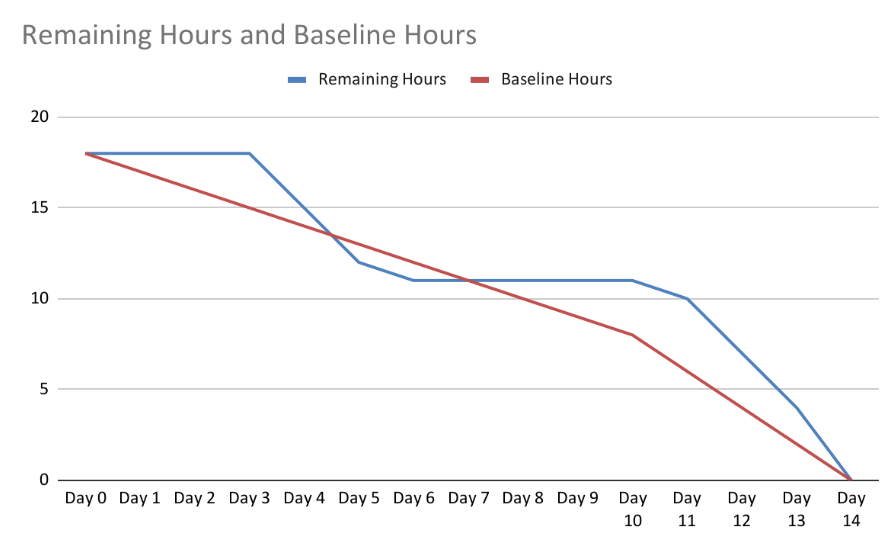
\includegraphics[width=0.5\textwidth]{images/burndown}
    \caption{Example sprint burn down chart}
\end{figure}

\subsubsection{Sprint Retrospective}
The sprint retrospective will be conducted as a team discussion at the end of each sprint. This meeting will reflect on success and areas for improvement, with all team members offering feedback. The key items will be the ways to improve, what did not work, and what did work well. The teammate responsible for that week's presentation will also be responsible for documenting the team's retrospective discussion.

\subsubsection{Individual Status Reports}
Over the sprint and during the group team retrospective, each teammate will document the hours they have worked on each task and discuss the task's completion. The relevant information will be documented individually by each teammate for their individual status report submission, including the teammate additionally responsible for the retrospective presentation.

\subsection{Closeout Materials}
The required materials will be submitted by the team in April 2025: 
\begin{itemize}
    \item Project poster
    \item CSE blog webpage
    \item Documents from 4316 and 4317
    \item Demo Videos, final demo \& extra footage
    \item Source code and documentation
    \item STL design files
    \item Circuit design files
\end{itemize}

\subsubsection{System Prototype}
The final system prototype will include the complete integration for the UR20 robot with a gripper and palletizing application. The prototype will be demonstrated by the UR20 robot palletizing boxes in ERB 335 in April 2025.
\subsubsection{Project Poster}
The project poster will include the project description, system architecture, results, and impact. It will follow standard poster dimensions (36"x48") and will be delivered in April 2025.

\subsubsection{Web Page}
The project webpage will include the project description, system requirements, demonstration videos, and deliverables. It will be provided at closeout in April 2025.

\subsubsection{Demo Video}
The video will show the UR20 robot in action performing palletizing tasks. B-reel footage will also be included for future video cuts. The video will be approximately 3-8 minutes long covering system setup, algorithms, and functionality.

\subsubsection{Source Code}
Source Code is written exclusively on the UR Teaching Pendant. Individual programs are saved and stored on the pendant, which is to be left with the UR20 to be accessible at all times. 

\subsubsection{Source Code Documentation}
Documentation will be written manually due to the nature of the UR20 Teaching Pendant.

\subsubsection{Hardware Schematics}
The hardware schematics will include wiring diagrams and any PCB layouts required for the integration of the gripper and accessory hardware.

\subsubsection{CAD files}
The project involves designing and printing a gripper, support components for the conveyor belt, and casing for the photoeye and camera. Tinkercad will be used for design. Final files will be provided in STL formats.

\subsubsection{Installation Scripts}
The programs will be handled by the teaching pendant and can be run from that source with little complication. The installation of the robot will largely involve physical installation in a location.

\subsubsection{User Manual}
A detailed user manual will be provided, including the setup steps in digital PDF format alongside a setup video demonstrating how the robot works. 